\section{Results}\label{sec:results}

As described in \autoref{sec:project}, the data of 5992 songs by German rap artists formed the basis of our research. For each song, information on the artists contributing, the album and the date of release was stored. This information was obtained using the Genius API. In addition, the final data set contains the lyrics to the corresponding song, which were treated using the preprocessing procedure described above and also saved in modified form.

The 5992 songs that remained after discarding non-German songs include 2094 participating artists and are spread among 1711 different albums. The number of artists involved includes not only primary artists, but also producers and featured artists. For example, the two producers Tim Wilke and David Kraft are the most frequent artists with 68 occurrences in the 5992 songs. The third most frequent artist in the available lyrics is Sido with 65 occurrences.

888 songs were declared as singles by Genius and were therefore not assigned to an album. This class also forms by far the largest share of the existing albums. The other existing albums are largely based on the limitation of song scraping to 15 songs per artist (see \autoref{sec:project}). The albums 'Instinkt' and 'Berlins Most Wanted' are both listed as 15 albums of one song. Only the album 'Liebeskummerparty' has 16 occurrences due to a song with a different artist.

\autoref{fig:number_songs} shows the temporal distribution of the songs. As it can be seen from the figure, the data set contains considerably fewer songs in the years 1998 to 2010 than in the period from 2010 to 2022. This could be due to the procedure for generating the data, which is essentially based on the predefined playlists from Spotify and the availability of various songs on the lyrics platform Genius. In addition, the number of artists in the Deutschrap genre has grown steadily over the years and was very low when the genre first emerged. The described disparity of the data affects the interpretability of the analyses. Details on this are explained in detail in the following sections.

\begin{figure}[!htb]
    \centering
    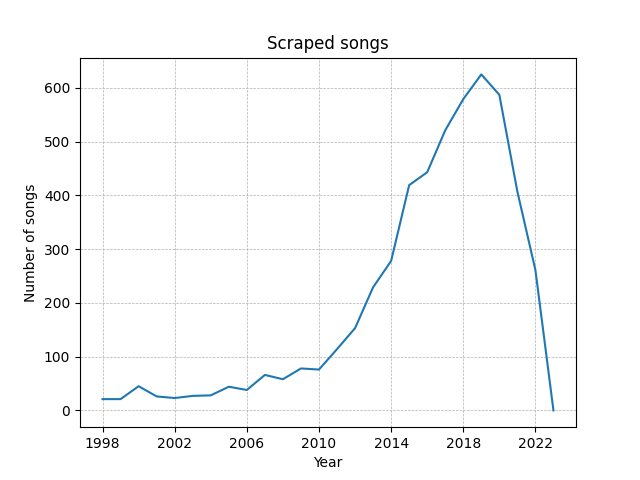
\includegraphics[width=0.8\textwidth]{figures/number_of_songs.png}
    \caption{Temporal distribution of scraped songs}
    \label{fig:number_songs}
\end{figure}

In the following, the results of the three different approaches to analyze the data will be presented in detail.

\subsection*{Occurrences check}

As outlined in \autoref*{sec:project}, an essential part of the task of the occurrences check was to elaborate a suitable dictionary for different categories, on the basis of which occurrences within the lyrics could be retrieved. After executing the process described in \autoref{sec:project} via Word2Vec and manual adjustment, the following quantities of words remained per category:

\def\arraystretch{1.2}
\begin{table}[!hbt]
    \centering
    \begin{tabular}{|l|l|}
    \hline
    \textbf{Category} & \textbf{Number of words} \\ \hline
    Misogyny        & 19 \\ \hline
    Violence        & 17 \\ \hline
    Anti-Semitism   & 14 \\ \hline
    Homophobia      & 14 \\ \hline
    Anti-disability & 13 \\ \hline
    Grief           & 12 \\ \hline
    Love            & 10 \\ \hline
    Racism          & 6  \\ \hline
    \end{tabular}
    \caption{Number of terms within each category of occurrences check}
    \label{tab:dictionary}
\end{table}

The different number of words per category is due to the fact that certain categories have fewer diverse terms than others. For example, the category misogyny contains a wide variety of vulgar terms for prostitutes, while the racism category almost exclusively contains the word 'nigger'.

The following \autoref{tab:occurrences_total} shows the absolute count of occurrences of the different categories in the entire data set. The categories love, misogyny and violence combine more than 85\% of all occurrences with 31451 of 36833 counted occurrences. 3628 of the examined songs contain at least one occurrence of the category love, which corresponds to about 61\% of the entire data set. The category violence was detected at least once in 3099 songs, approximately 52\% of all songs. We detected misogynistic terms in 2431 songs, about 41\% of the population. In 757 songs, no occurrences of the predefined categories could be found.

\begin{table}[!htb]
    \centering
    \begin{tabular}{|l|l|}
    \hline
    \textbf{Category} & \textbf{Number of occurrences} \\ \hline
    Love              & 12098                          \\ \hline
    Violence          & 10251                          \\ \hline
    Misogyny          & 9102                           \\ \hline
    Racism            & 2051                           \\ \hline
    Grief             & 1294                           \\ \hline
    Homophobia        & 1253                           \\ \hline
    Anti-disability   & 546                            \\ \hline
    Anti-semitism     & 238                            \\ \hline
    \end{tabular}
    \caption{Absolute count of occurrences of investigated categories}
    \label{tab:occurrences_total}
\end{table}

For further analysis, we examined the behaviour of the occurrences based on the release date of the songs. Due to the previously mentioned bias in the number of songs per year, we normalised the number of occurrences per year. \autoref{fig:occurrences_time_series} shows the development of the occurrences over the examined period 1998 to 2022. The different lines show the normalised number of occurrences per song for each category. The different categories are marked with different colours. It can be observed that especially around the year 2003, a relatively large number of songs contained violent and misogynistic terms, but at the same time also many on the subject of love. Until 2010, the occurrences of the three mentioned categories decrease to an average level of 3 occurrences per song. They maintain this level in the following years up to 2022. The other categories are less prevalent throughout the entire study period: Only the categories homophobia in 2006 and racism in 2003 exceed the mark of 1 average occurrence per song.

\begin{figure}[!htb]
    \centering
    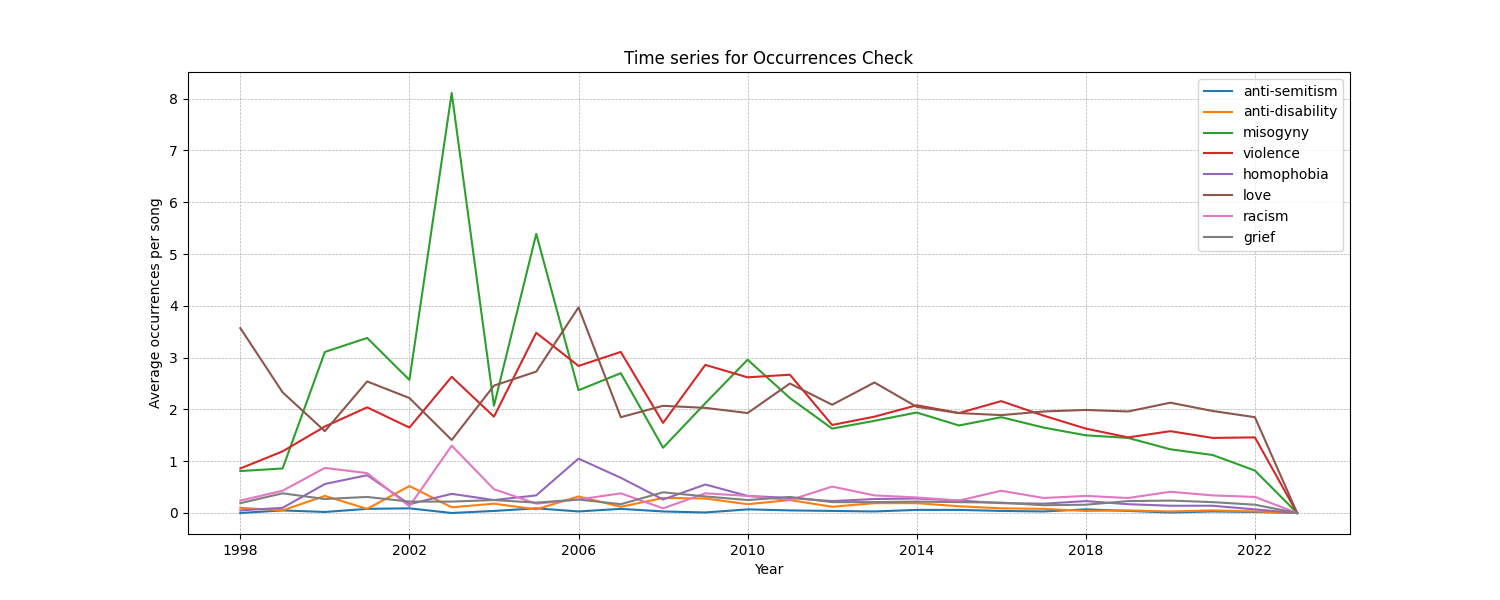
\includegraphics[width=\textwidth]{figures/time_series_occurrences.png}
    \caption{Time series analysis of counted occurrences}
    \label{fig:occurrences_time_series}
\end{figure}

\subsection*{Sentiment analysis}

For the analysis of the two described methods for sentiment analysis (German Sentiment Bert and Toxicity), we studied the distributions of the values across the data set. \autoref{fig:sentiment} shows the distribution of the values of the German-Sentiment-Model according to the described procedure in \autoref{sec:project}. Similarly, \autoref{fig:toxicity} shows the distributions of the values of the toxicity classifier. The left graph of the figure represents a histogram of the distribution over the complete investigation period. The right graph in contrast shows the temporal course of the values. The middle blue line within this graph corresponds to the median of the examined songs within each year, the surrounding shaded area contains all data that falls into the range of the 25\%- to 75\%-quantile. In other words, 50\% of the songs examined have a sentiment or toxicity value within the shaded area.

In general, one can observe for the sentiment analysis via German Sentiment Bert that a negative sentiment prevails in the songs. The median of all data is -0.40, the 25\% quantile is -0.52 and the 75\% quantile is -0.27. The clustering of data in this range can also be gathered from the histogram in \autoref{fig:sentiment}. Only 263 songs were assigned a sentiment greater than 0, which corresponds to a share of 4.4\% of all the songs examined. 

The time series analysis of the sentiment data on the right-hand side of \autoref{fig:sentiment} reveals no meaningful change in the sentiment of the songs studied over the research period. The median decreases slightly from -0.36 in 1998 to -0.42 in 2022. The lowest median can be found in 2009 with a value of -0.47, and the highest median in 2003 with a value of -0.31.

\begin{figure}[!htb]
    \centering
    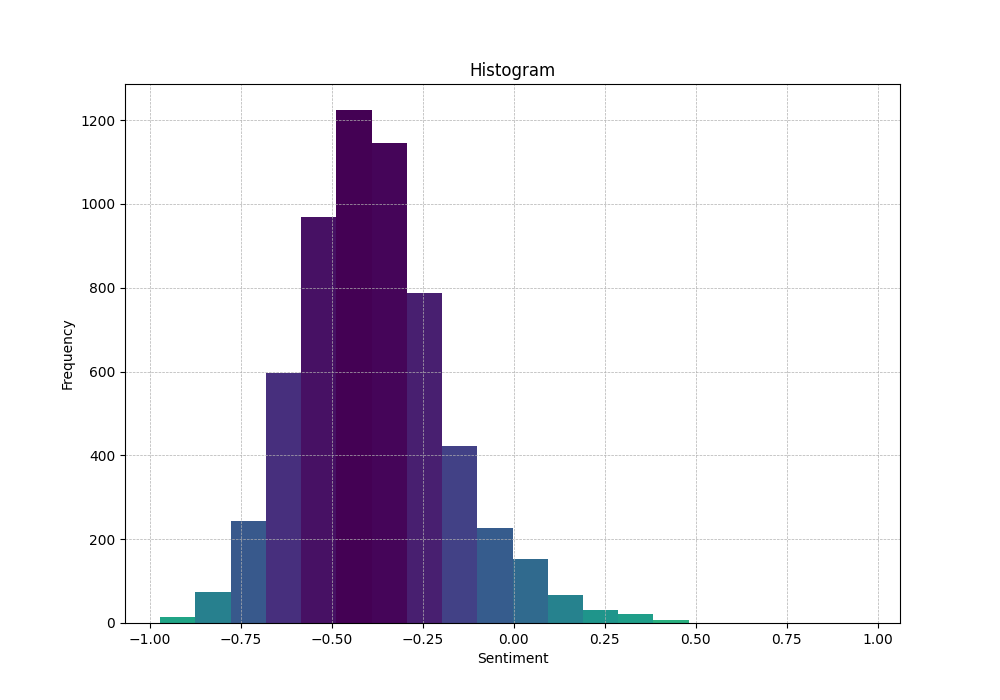
\includegraphics[width=0.49\textwidth]{figures/sentiment_histogram.png}
    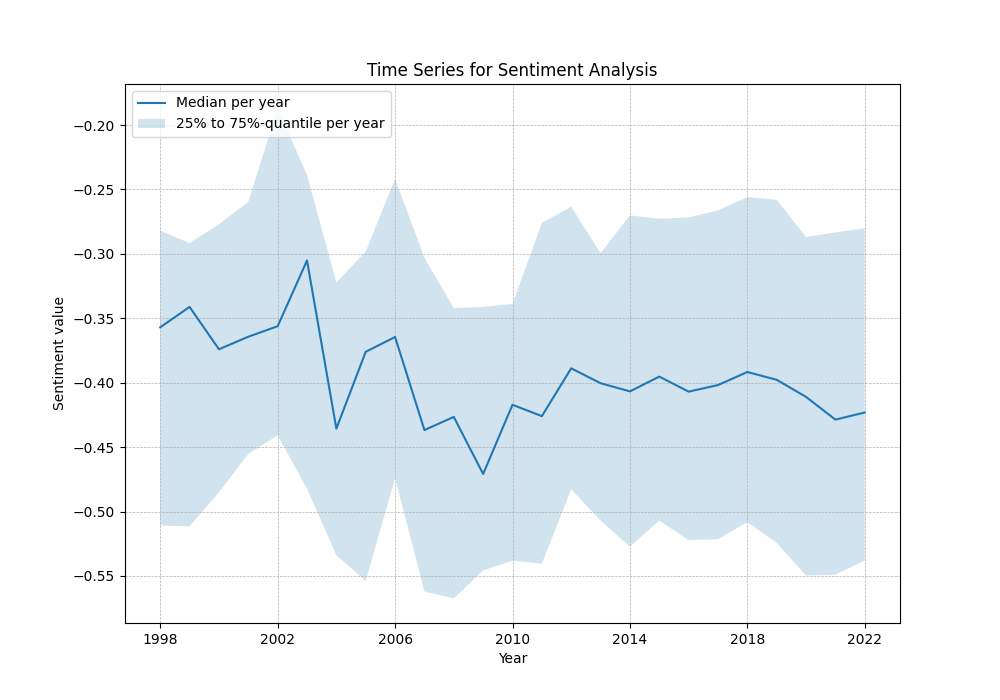
\includegraphics[width=0.49\textwidth]{figures/time_series_sentiment.png}
    \caption{Distribution of results regarding German-Bert-Sentiment analysis}
    \label{fig:sentiment}
\end{figure}

The toxicity analysis also shows a rather one-sided distribution of the examined data, as the histogram on the left side of \autoref{fig:toxicity} shows. 1100 songs are classified with a positive value by the toxicity classifier, i.e. they are classified as rather toxic. This corresponds to a share of 18\% of the population. The median of the toxicity values of all songs is -0.34, the 25\% quantile is -0.60 and the 75\% quantile is -0.08. The development over time, shown on the right side in \autoref{fig:toxicity}, shows a slight downward trend over the years. In other words, songs are becoming less toxic based on the toxicity analysis, but with the starting level in the 2000s already being classified as non-toxic.

\begin{figure}[!htb]
    \centering
    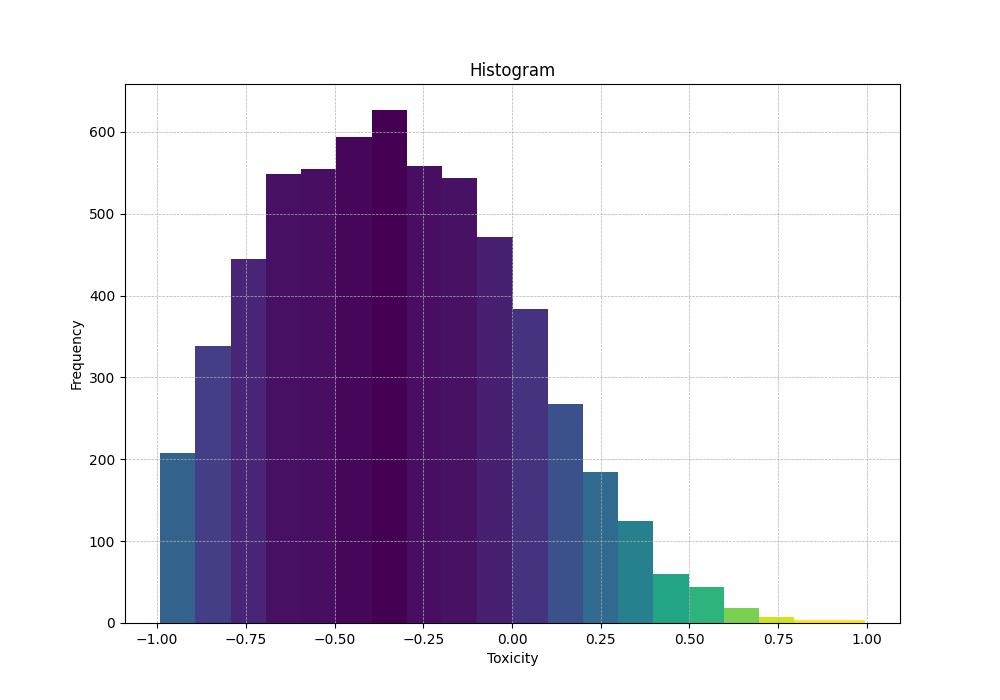
\includegraphics[width=0.49\textwidth]{figures/toxicity_histogram.png}
    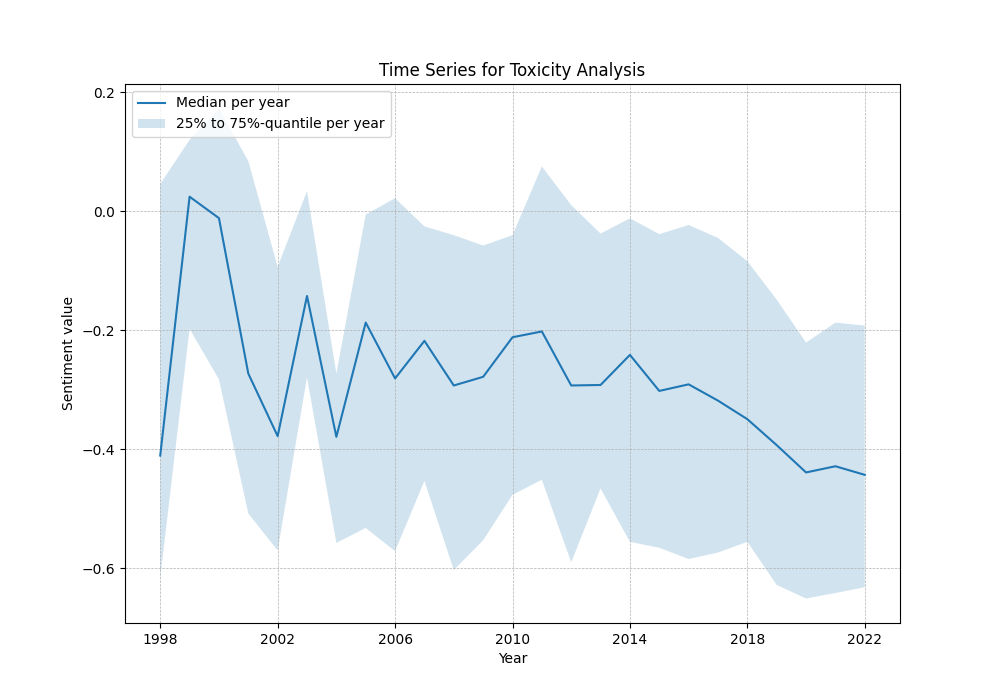
\includegraphics[width=0.49\textwidth]{figures/time_series_toxicity.png}
    \caption{Distribution of results regarding Toxicity analysis}
    \label{fig:toxicity}
\end{figure}

For a further analysis of the two methods of sentiment analysis, we compared the results of the two classifiers. Pearson's correlation coefficient provides insights into a possible dependency of the data. The result of the two variables German Sentiment Bert and Toxicity is -0.13.



\subsection*{Zero-shot classifier}

The classification via zero-shot method (see \autoref{sec:project}) provides probabilities for the given classes per song. Figure \autoref{fig:zero-shot} shows the distribution of classes across the data set. The graph on the left only considers the most likely class per song and ignores all probabilities of the other classes. It thus corresponds to a one-hot-encoded classification to a single category per song. As one can see from the graph, the class 'positive' is the most prevalent with 2149 songs assigned to it, followed by the category 'friendly' with 1732 occurrences and 'violent' with 935 occurrences. The categories 'affectionate', 'neutral' and 'mysoginistic' were selected as the most likely category only a few times. 'Racist' and 'homophobic' were not assigned to any song with the highest probability.

Looking on the right side of \autoref{fig:zero-shot}, one gets insight into the summed probabilities of the categories. This reveals a slightly differentiated picture: The categories 'positive' and 'friendly' remain at the top, but with a smaller difference compared to the one-hot-encoded approach on the left side of \autoref{fig:zero-shot}. The categories 'affectionate', 'violent', 'neutral' and 'mysoginistic' gain more importance in this view. 'Racist' and 'homophobic' are still relatively underrepresented.


\begin{figure}[!htb]
    \centering
    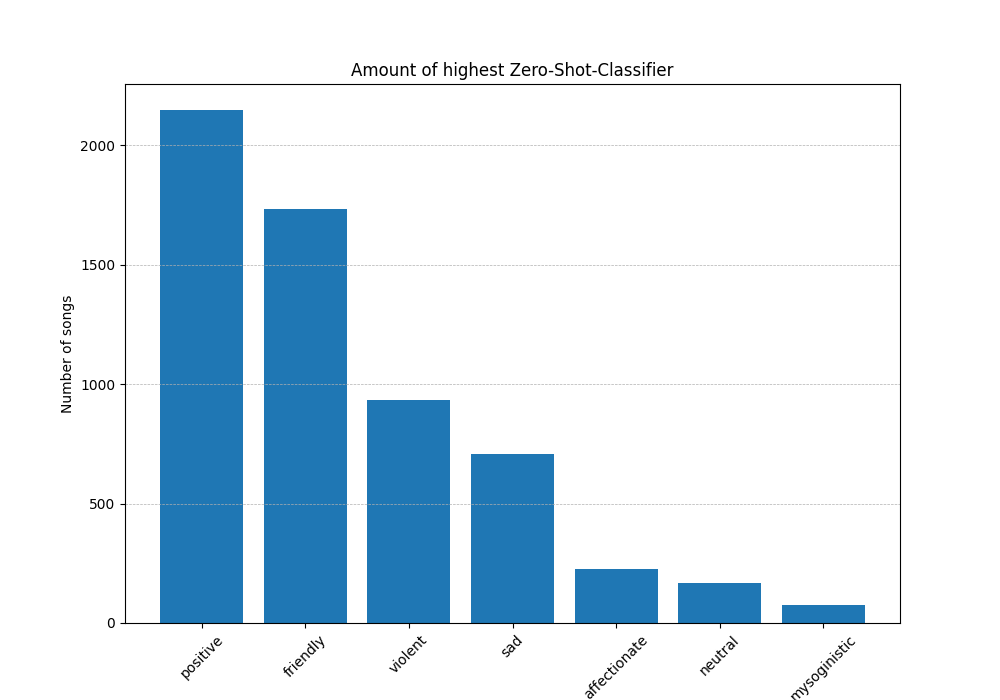
\includegraphics[width=0.49\textwidth]{figures/overall_score_binary_zero_shot.png}
    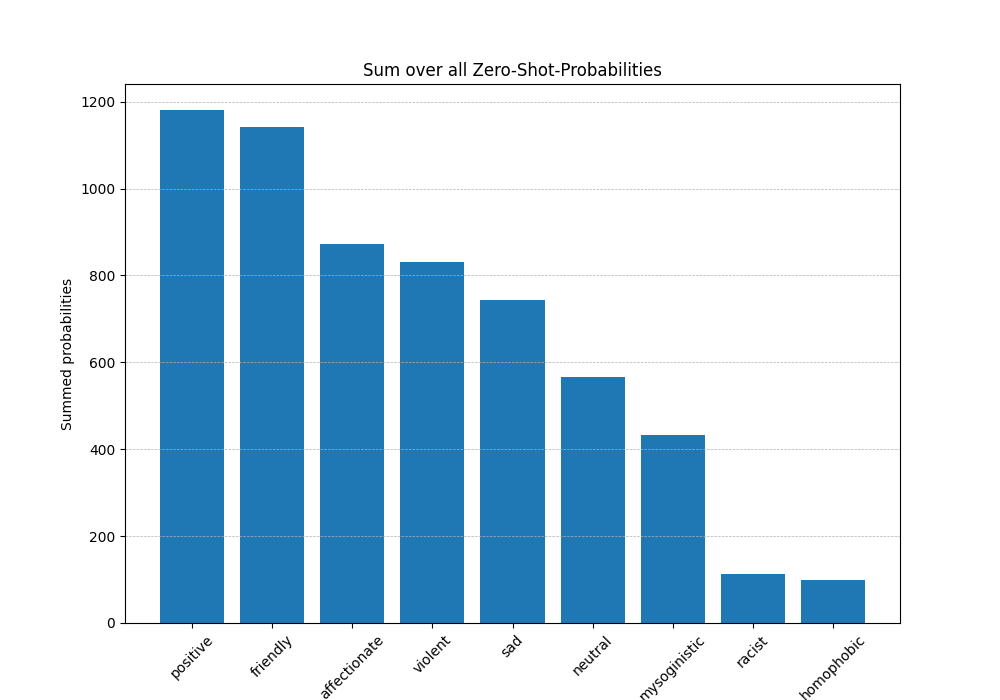
\includegraphics[width=0.49\textwidth]{figures/overall_score_zero_shot.png}
    \caption{Distribution of categories regarding zero-shot classifier}
    \label{fig:zero-shot}
\end{figure}

The following diagram in \autoref{fig:zero-shot2} provides an in-depth view of the development of the data over time with regard to the zero-shot classification: Four-year periods in the study period 1998 to 2022 are each shown with the three predominant categories in relation to the summed probabilities of the classifier. Due to the bias in the number of songs in the different periods (see \autoref{fig:number_songs}), the sum of the probabilities was divided by the number of songs per period. Over the period studied, the values of the two most probable categories, 'friendly' and 'positive', are close to each other and continue to converge. Until 2014, the third most relevant category is 'violent', before it is replaced by 'affectionate'. The average probability for the third-highest category is between 12.5\% and 15\%. 

\begin{figure}[!htb]
    \centering
    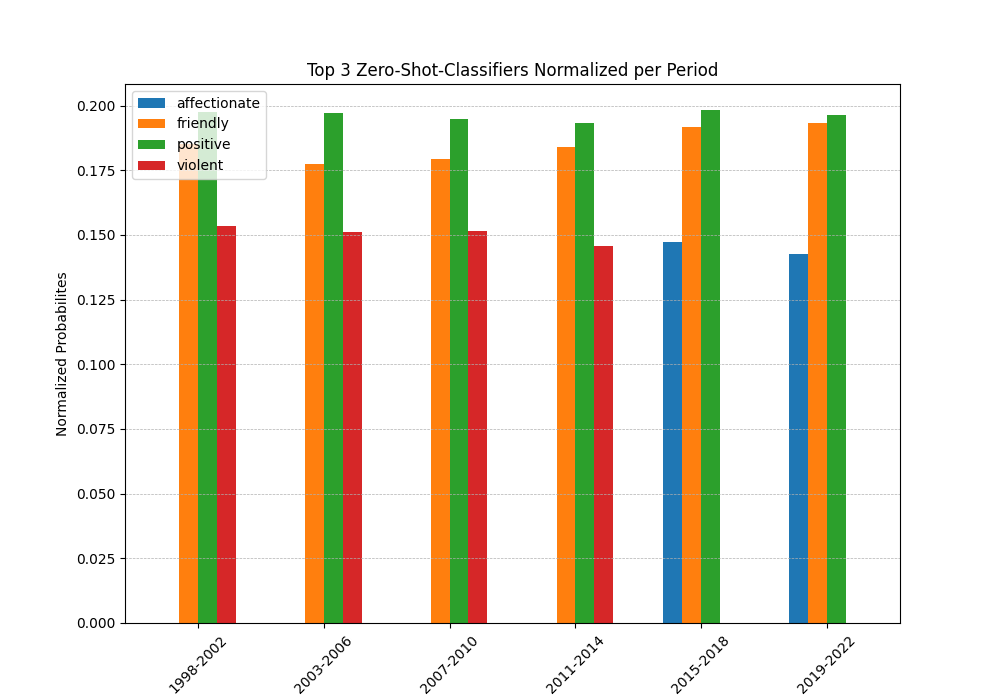
\includegraphics[width=\textwidth]{figures/top_3_time_series_zero_shot.png}
    \caption{Time series analysis for the top 3 prevalent categories of zero-shot-classifier}
    \label{fig:zero-shot2}
\end{figure}

\subsection*{Evaluation}

In order to be able to classify the results and assess their quality, we have developed methods for evaluating the results. No evaluation was carried out for the occurrence test, as this method is based on pure counting and therefore only allows for misinterpretation to a limited extent. For the other methods, we faced the challenge that the data used was not labelled as it should be for a complete evaluation. Our dataset was self-acquired, so we had no data against which to compare the results of our methods.

One of the options we considered at this stage was to use ChatGPT \ OpenAI's Playground platform to automate the very time-consuming process of labelling the songs. Unfortunately, we encountered a few problems in the process. One of them was the inconsistency of the labelling, i.e. the same lines were interpreted and classified differently each time they are given as input to the AI. However, this might be something a human could do as well, one could interpret things from different perspectives at different times. One even more major issue was the recognition of swear words in OpenAI, of which there are many in German rap. OpenAI doesn't allow profanities in its prompts, thus the prompts are blocked. This has completely ruled out this option for us.


We therefore decided to manually label about 70 songs, of which we had an equal number from each classes of the three different methods used, so we were able to equally evaluate the efficiency and accuracy of the methods in relation to the different labels we had. During the labelling process, we realised how difficult it is even for people to assign a label, be it a positive, negative or even more specific label (like racist, misogynistic, etc.). Many biases could influence the decision, and the songs leave a lot of room for different perspectives and interpretations of their content. 

So the task of labeling the songs itself proved to be very challenging, which is why we decided not to give the chosen label a percentage probability, but to simply classify them in a binary way. So we decided to ignore the exact probabilities that the different methods assigned to the different possible classes and consider them as a binary classification.

For the evaluation, we've decided to use a Confusion Matrix and consider the F1 Score.
We've compared our labels with the predictions of the different methods in the following manner:
\begin{itemize}
    \item Sentiment Analysis (German Sentiment Bert): We mapped any negative sentiment, i.e. probability less than 0, to -1 and any positive sentiment to 1.
    \item Toxicity Analysis: We did the same approach as for German Sentiment Bert: Mapping was done to -1 for not toxic songs and 1 for toxic songs.
    \item Zero-shot Classification: We omitted the probabilities and took the class with the highest probability as the label of the song.
\end{itemize}

The confusion matrices for the different methods can be found below:

\begin{table}[!htb]
    \centering
    \begin{tabular}{l|llll}
     & Precision & Recall & F1-Score & support \\ \hline \hline
    negative & 0.63 & 0.98 & 0.77 & 42\\
    positive & 0.67 & 0.08 & 0.14 & 26 \\ \hline
    accuracy & & & 0.63 & 68\\
    macro avg & 0.63 & 0.53 & 0.45 & 68 \\
    weighted avg & 0.64 & 0.63 & 0.53 & 68\\
    \end{tabular}
    \caption{Confusion matrix for Sentiment Analysis (German Sentiment Bert)}
    \label{tab:confusion_matrix_sentiment}
\end{table}

\begin{table}[!htb]
    \centering
    \begin{tabular}{l|llll}
     & Precision & Recall & F1-Score & support \\ \hline \hline
    neutral & 0.53 & 1.00 & 0.69 & 35\\
    toxic & 1.00 & 0.06 & 0.11 & 33 \\ \hline
    accuracy & & & 0.54 & 68\\
    macro avg & 0.77 & 0.53 & 0.40 & 68 \\
    weighted avg & 0.76 & 0.54 & 0.41 & 68\\
    \end{tabular}
    \caption{Confusion matrix for Toxicity Analysis}
    \label{tab:confusion_matrix_toxicity}
\end{table}

\begin{table}[!htb]
\centering
\begin{tabular}{l|llll}
 & Precision & Recall & F1-Score & support \\ \hline \hline
neutral & 0.22 & 0.22 & 0.22 & 9\\
affectionate & 0.70 & 0.78 & 0.74 & 9 \\ 
violent & 0.67 & 0.40 & 0.50 & 15\\
racist & 0.00 & 0.00 & 0.00 & 1\\
homophobic & 0.00 & 0.00 & 0.00 & 0\\
misogynist & 0.33 & 0.60 & 0.43 & 5\\
friendly & 0.00 & 0.00 & 0.00 & 0\\
positive & 0.36 & 0.50 & 0.42 & 8\\
sad & 1.00 & 0.48 & 0.65 & 21\\ \hline
accuracy & & & 0.47 & 68\\
macro avg & 0.41 & 0.37 & 0.37 & 68 \\
weighted avg & 0.65 & 0.47 & 0.52 & 68\\
\end{tabular}
\caption{Confusion matrix for Zero-shot Classifier}
\label{tab:confusion_matrix_zero_shot}
\end{table}

\newpage







